\section{Background}
In this section some basics concepts related to the human walking are introduced. Later they will
be applied to the robot walking 
\subsection{Locomotion in human being}
The \emph{gait cycle} is defined as the time between two successive foot contact of the same limbs,
it can be divided in two phases, the \emph{Stance Phase}  and the \emph{Swing phase}.
For analyzing gait cycle one foot is taken as reference and its movements studied.
The Stance phase is the part of a gait cycle during which the foot remains in contact with the
ground, it constitutes about the $60\%$ of the gait cycle. In this phase five parts can be
distinguished:
\begin{itemize}
\item [-]\emph{Initial contact}: Instant the foot contacts the ground;
\item [-]\emph{Loading response}: Time period between the initial contact phase and the instant
  when the other foot lifts the ground;
\item [-]\emph{Mid stance}: Time interval from the end of the Loading response phase to the time
  when both ankles are aligned in the frontal plane;
\item[-]\emph{Terminal stance}: Period from ankles alignment to the contact of the swinging foot;
\item[-]\emph{Pre swing}: Time interval between the end of the terminal stance phase and the instant
  when the foot lifts from the ground.
\end{itemize}
The Swing phase is the phase of the gait during which the reference swings. It takes about $40\%$ of the gait cycle. Three parts can be distinguished:
\begin{itemize}
\item [-]\emph{Initial swing}: Phase during which the reference foot is lifted from the ground
  to position of maximum  knee flexion;
\item [-]\emph{Mid swing}: Time period between the initial contact phase and the instant when the other foot lifts the ground;
\item[-]\emph{Terminal swing}: Following vertical tibia position to just prior to initial contact.
\end{itemize}
Last but not least the concepts of Double and Single support are introduced. The first one refers to
the period during which boot feet are in contact with the ground while the other refers to interval when only one foot is in contact with the ground.
\par
In figure \ref{fig:gait-cycle} all the phases described above are shown. For each phase the type of support (single or double) is specified.
\begin{figure}[!ht]
  \centering
  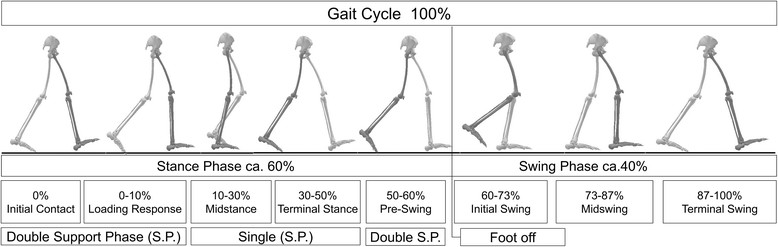
\includegraphics[scale=0.45]{gait-cycle.png}
  \caption{Classification of a human gait cycle. Image downloaded from \cite{Merker2015}. \label{fig:gait-cycle}}
\end{figure}
\par
In the following subsection the concepts described will be applied to the robot walking.
\subsection{Locomotion in robotic systems}
In robot locomotion the gait cycle described in the above section is simplified,
and the phases described are condensed in more general groups.
The walking task can be easy summarize using the \emph{walking cycle}
(Figure \ref{fig:walking_fsm}), it embeds all the phases of the human locomotion
shown in the figure \ref{fig:gait-cycle}. 
\begin{figure}[!ht]
  \centering
  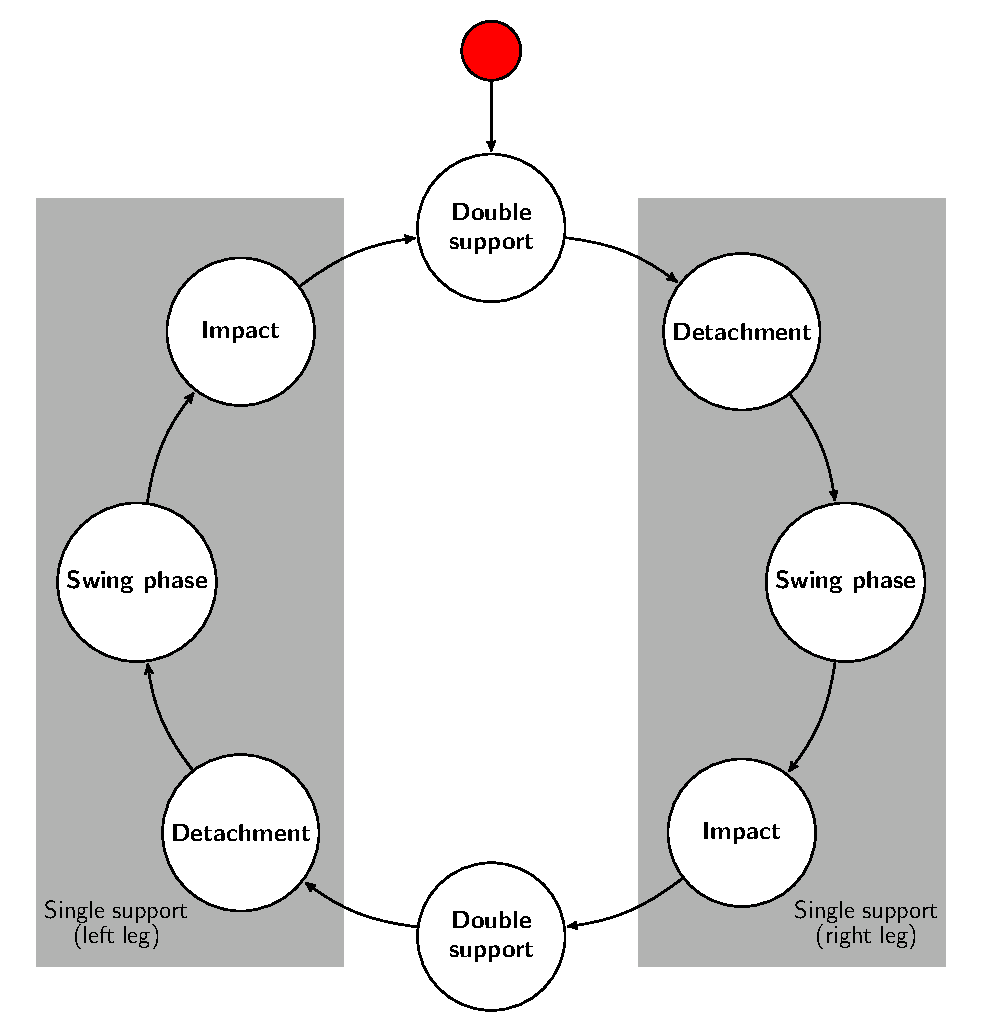
\includegraphics[scale=0.4]{walking_fsm}
  \caption{Walking cycle state machine. \label{fig:walking_fsm}}
\end{figure}
\par
The cycle can be split in two main phases, the Double support and the Single support ones.
The first one embeds the initial contact, the loading response and the pre swing phases while the
single support phase embeds the others.
During the SS phase the movement of the swing foot (i.e. the non reference foot)
is usually split in three sub-phases, \emph{detachment}, \emph{swing} and \emph{impact}.
More detailed:
\begin{itemize}
\item[-]\emph{Detachment}: Instant when the foot lifts from the ground;
\item[-]\emph{Swing}: this phase embeds the Initial swing, the mid swing and the terminal swing
  stages of the human walking;
\item[-]\emph{Impact}: Instant the foot contacts the ground.
\end{itemize}
In the following of this report only the single support phase is analyzed. Initially from the point
of view of the reference foot and the robot center of mass. Later the movement of the swing foot is
studied. 
\newpage
